\chapter{Punto de impacto del cono \cher{} sobre la tierra}
\label{ap:intPlanCon}

	La superficie de impacto del cono \cher{} y la tierra puede pensarse de manera abstracta como el problema de hallar la intersección entre un cono y un plano, tal como se esquematiza en la figura \ref{fig:conoInt}.
	\begin{figure}[ht!]
		\centering
		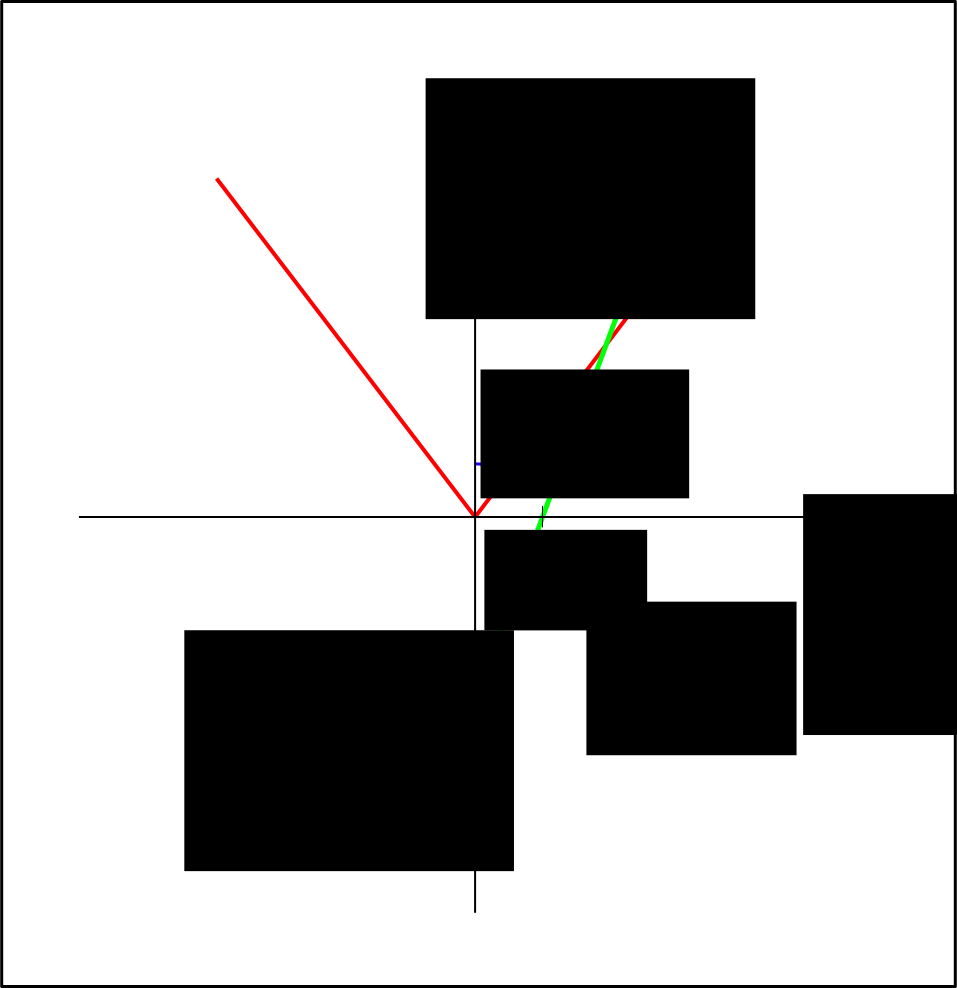
\includegraphics[width=0.45\textwidth]{./fig/appendix/conoInt}
		% curveEarthSketch.png: 2404x1199 pixel, 150dpi, 40.70x20.30 cm, bb=0 0 1154 575
		\caption{\label{fig:conoInt}
		Esquema del problema abstracto, intersección de un cono y un plano.
		}
	\end{figure}
	Las ecuaciones \ref{eq:plano1} y \ref{eq:cono1} corresponden al plano y al cono que nos interesan, respectivamente.
	\begin{equation}
	z=\frac{x-h}{\tan \beta}
	\label{eq:plano1}
	\end{equation}
	\begin{equation}
	z=\frac{x^2+y^2}{\tan^2 \alpha}
	\label{eq:cono1}
	\end{equation}
	Dado que se busca el ancho $y(z)$ de dicha intersección hay que despejar $x$ de la ecuación \ref{eq:plano1} y reemplazarla en \ref{eq:cono1}. 
	El resultado es el de la ecuación \ref{eq:int1}.
	\begin{equation}
	\tan^2\alpha\ z=y^2+(h+\tan \beta\ z)^2
	\label{eq:int1}
	\end{equation}
	Luego, expandiendo y despejando se obtiene la ecuación para el ancho \ref{eq:int2}. 
	\begin{equation}
	y^2=(\tan^2 \alpha-\tan^2 \beta) z^2 - \tan\beta\ h z - h^2
	\label{eq:int2}
	\end{equation}
	Esta, no tiene solución real si $h>0$ y $\beta>\alpha$.
	Finalmente, para volver a nuestro problema físico, hay que reemplazar:
	\begin{itemize}
	\item $y \rightarrow w$
	 \item $\alpha \rightarrow \theta_{cher}$
	 \item $\beta \rightarrow \theta - \frac{\pi}{2}$
	 \item $h \rightarrow \frac{h_{max}}{\sin{\theta}}$
	 \item $z \rightarrow l-l_{max} = \frac{d}{\sin \theta} -l_{max}$
	\end{itemize}
	obteniendo finalmente la ecuación \ref{eq:conewidth}.
